In der Abbildung \ref{fig:dateflowVScodedep} sieht man ein Beispiel von einer Anwendung, die die von der Konsole ankommenden Zahlen quadriert und das Ergebnis zurückgibt.
                
\begin{figure}[H]
    \centering
    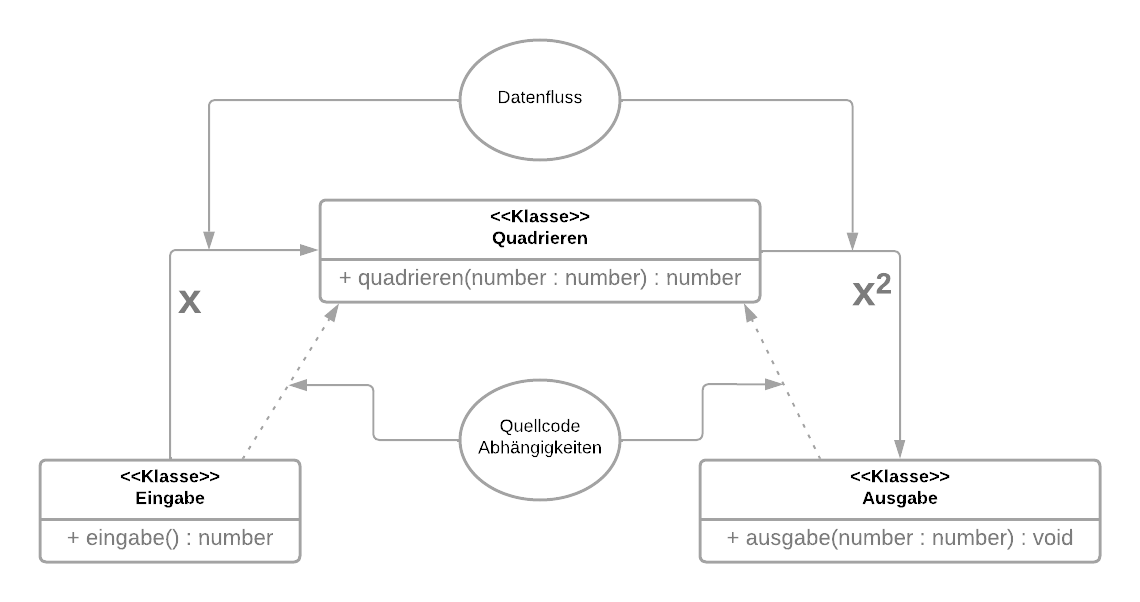
\includegraphics[width=1\textwidth]{./images/DepInj_1.png}
    \caption{Datenfluss und Quellcode Abhängigkeiten}
    \label{fig:dateflowVScodedep}
    \source{Eigene Quelle}
\end{figure}

Die Funktion \textbf{Quadrieren} ist in dem Fall befindet sich auf einem höheren Niveau als Eingabe und Ausgabe, 
da das Quadrieren einer Zahl soll unabhängig von der Eingabe und Ausgabe sein.

Würde man aber bei der Ausgabe die Eingabeparameter von \textbf{number} auf \textbf{string} ändern, 
so müsste man auch die Ausgabe von Quadrieren von \textbf{number} auf \textbf{string} ändern.
Dies könnte auch eine weitere Kette an Anderungen im Programm auslösen. 
Zum Beispiel müssen auch die Unittests von \textbf{Quadrieren} geändert werden.
Somit ist \textbf{Quadrieren} abhängig von der \textbf{Ausgabe}

Das Problem lässt sich mittels Dependency Injection lösen.
In OOP Sprachen kann man dafür ``Interface'' benutzen.

Die Lösung wurde dann so aussehen. 
\begin{figure}[H]
    \centering
    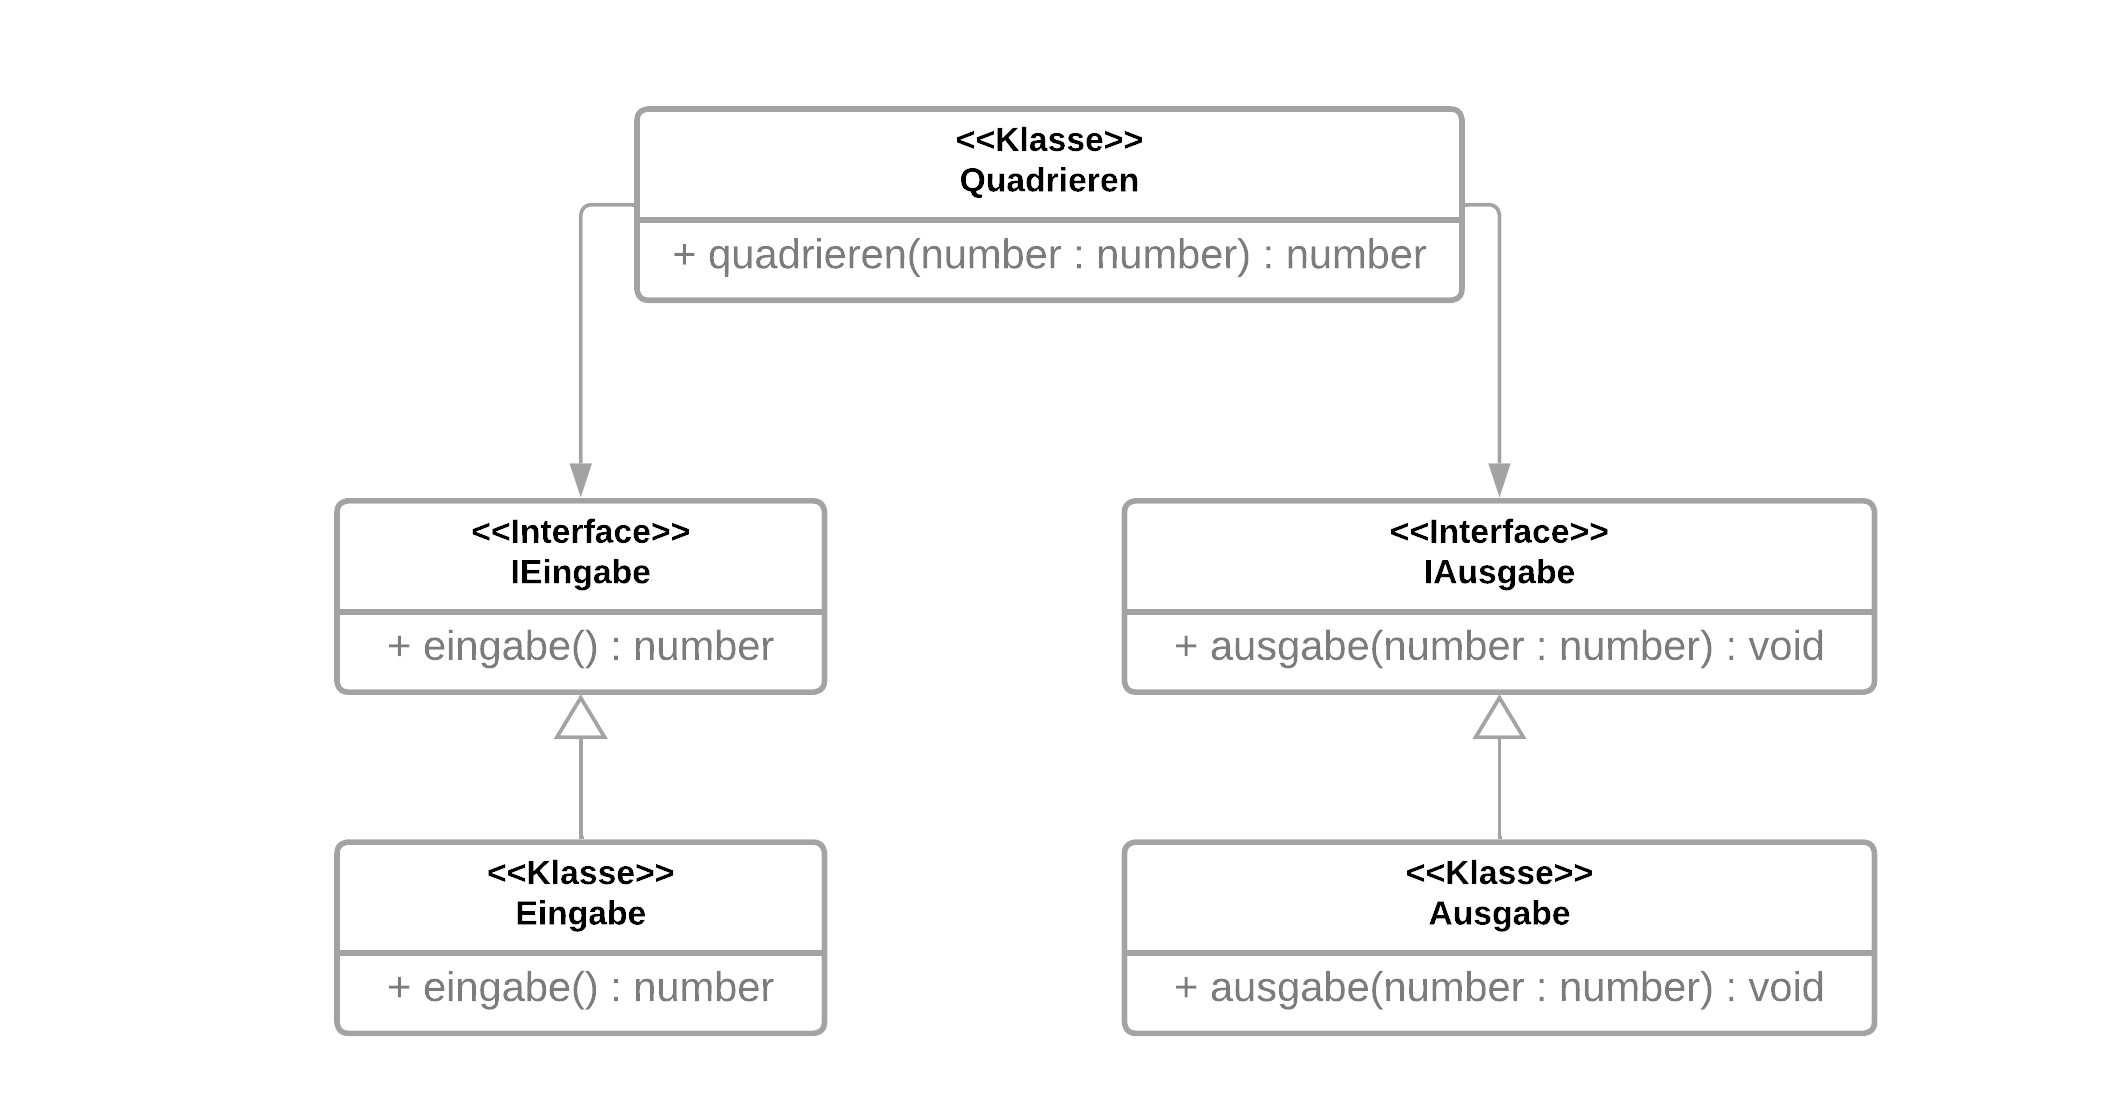
\includegraphics[width=1\textwidth]{./images/DepInj_2.png}
    \caption{Entkopplung der Abhängigkeiten}
    \label{fig:flow around cylinder}
    \source{Eigene Quelle}
\end{figure}

Dies lässt sich mit \textbf{Interface} (für OOP Sprachen) umsetzen, 
in dem es frühestens bei der Initialisiereung der \textbf{Quadrieren} 
Klasse das jeweilige Eingabe und Ausgabe Objekt übergeben wird.

Somit lässt sich die Funktion \textbf{Quadrieren} mit gefälschten Eingabe- und Ausgabeklasse mit Unit tests getestet werden.

Wenn man alle Klassen über Interface miteinander verbindet, 
ist es möglich, dass die Umgebung von jeder einzelnen Klasse bei den Unittests gefälscht
wird und somit das Schreiben von Unittests sehr einfach wird. 

Interfaces können sich natürlich auch ändern und dann muss man auch alle davon betroffenen Objekte entsprechend ändern, 
jedoch das passiert deutlich seltener als Änderung einer Klasse.

Auch mit Dependency Injection lassen sich externe Schnittstellen wie Datenbank oder Netzwerkschnittstellen schnell austauschen, 
denn man muss nur eine Klasse schreiben, die das Interface implementiert.